
\begin {figure*}
 \centering
  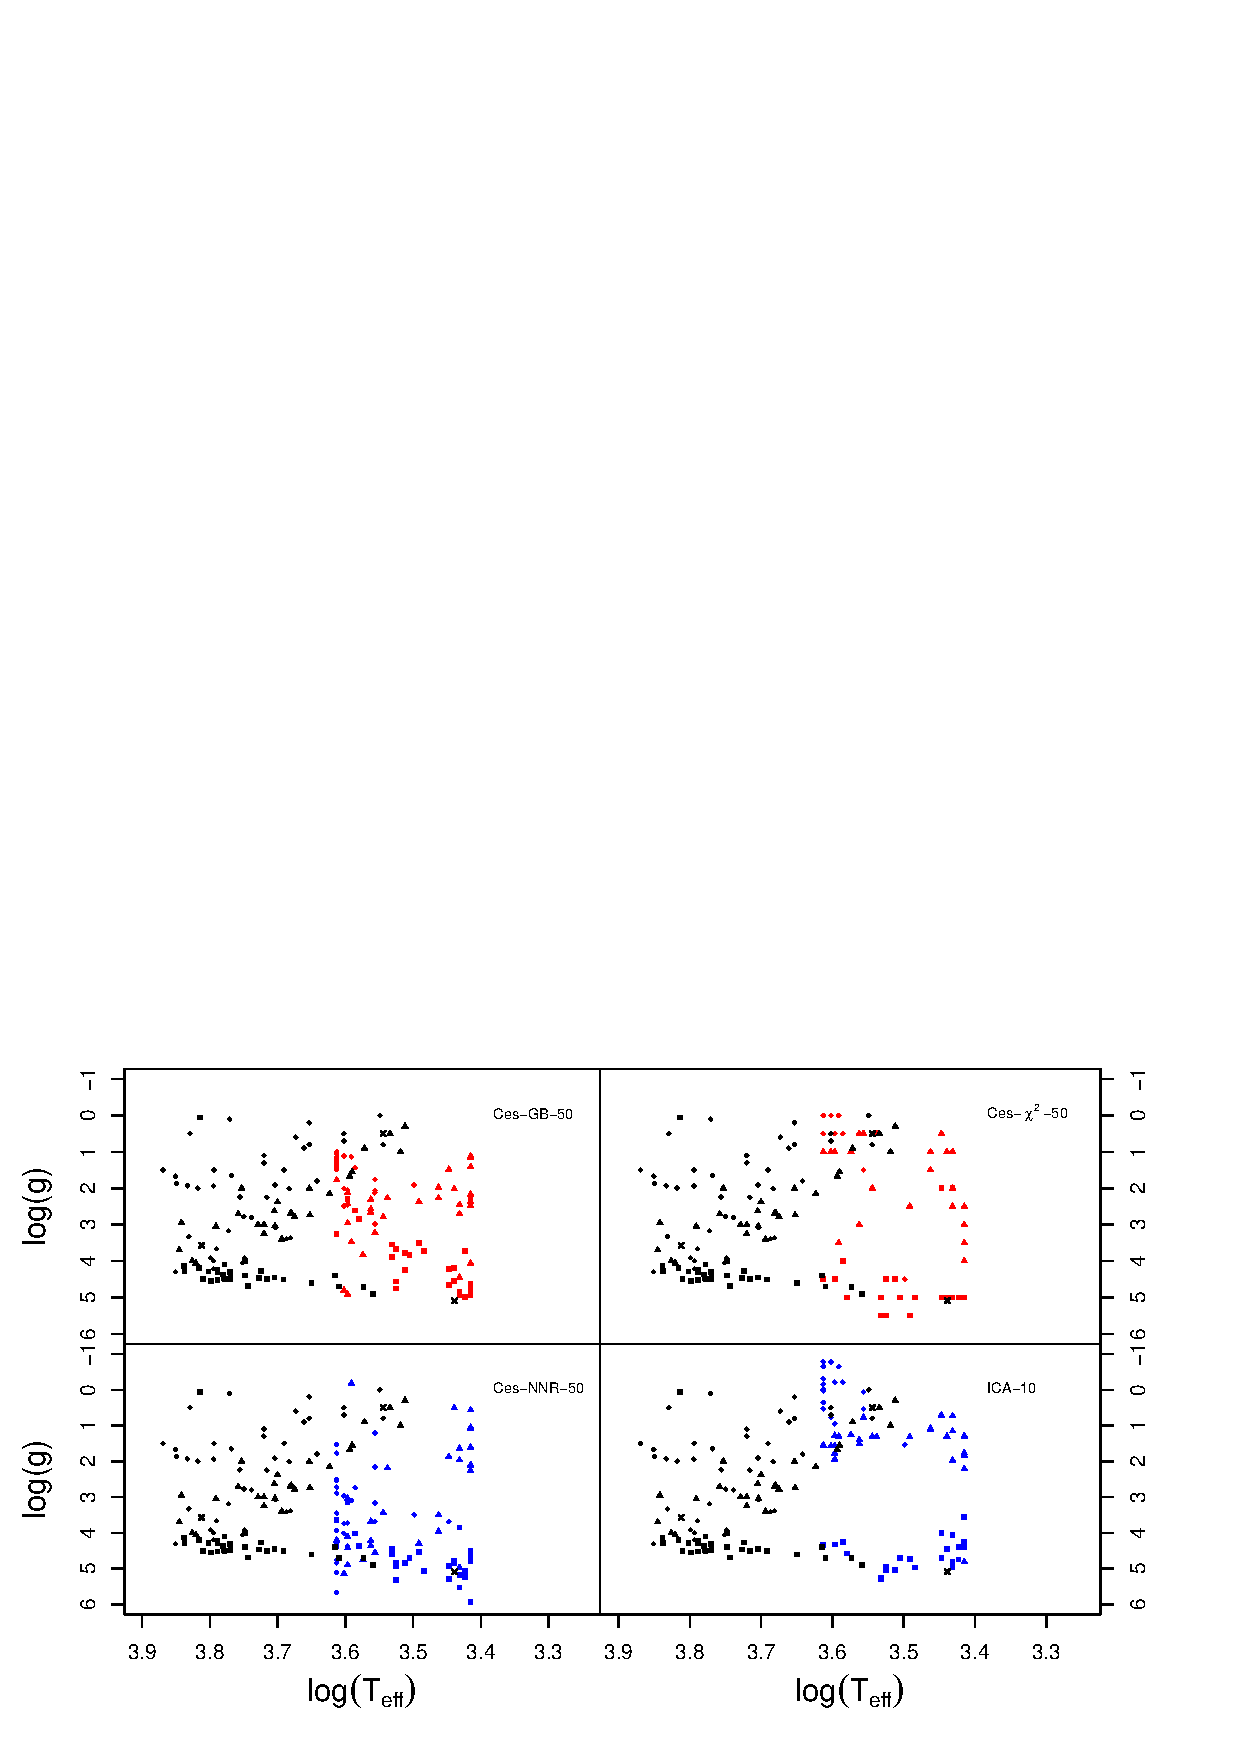
\includegraphics[width=\textwidth]{figs/irtf-figs/irtf-Cesseti.pdf}
  \caption{$\log(T_{eff})$--$\log(g)$ diagrams produced by the CES-KNN
    (SNR=$\infty$) effective temperatures, and gravities derived with
    the CES-GB (SNR=50), CES-$\chi^2$ (SNR=50), CES-NNR (SNR=50), and $ICA-10$
    models (clockwise, starting from the top left plot).}
 \label{fig:irtf-ces}
\end {figure*}

{\bf TODO 12: Discuss differences in ICA-10 predictions in GA and
  CES. See email from Joaquín.}
 
For metallicities, we again find that the only feature space that
results in reasonable results is based on ICA projections and
SNR=10. Comparison of the correlation coefficients of the various
regression results with the literature values shows no significant
difference between the GA-based features and those taken from
\cite{cesetti}. Therefore, neither set is competitive with the ICA
projections. In Fig. \ref{fig:irtf-ces-met} we show the results of the
regression technique that results in the highest correlation with the
literature values (RF-50).

\begin {figure}
\centering
\includegraphics[width=\textwidth]{figs/irtf-figs/M-CES.pdf}
\caption{Comparison of the CES-RF (SNR=50) regression model
  predictions with the estimates of the metallicity in the
  literature. The symbols and colours are the same as in Figure
  \ref{MIRTF_ICA_10}.}
\label{fig:irtf-ces-met}
\end {figure}
